\newpage
\chapter{Transformation Daten zu Netzwerk}
Ziel dieses Forschungsprojektes ist es unter anderem verschiedene Algorithmen, zur Ausrei�er Erkennung in Netzwerken, auf andere Datenformen anzuwenden. Hierbei werden haupts�chlich Zeitreihen untersucht. Um die Algorithmen auf andere Datenformen anwenden zu k�nnen, m�ssen die Daten zun�chst in ein Netzwerk umgewandelt werden. Die Voraussetzung daf�r dass Daten in ein Netzwerk umgewandelt werden kann ist, . Dieser Schritt wird in diesem Kapitel erl�utert. Exemplarisch wird der Vorgang an der Transformation von Zeitreihen aufgezeigt. 


\label{chap:trsnsNeti}
Der erste Schritt der Transformation ist, zun�chst die Distanz zwischen den einzelnen Elementen des Zeitintervalls berechnet. Hierzu wird auf das in \citep[vgl.][S.~2-3]{10.3389/fphy.2019.00194} vorgestellte Distanzma� zur�ckgegriffen. Insofern f�r p = 2 eingesetzt wird, handelt es sich um die euklidische Distanz. Die Abst�nde bilden die Kantengewichte zwischen den jeweiligen Elementen im Netzwerk. Die Elemente der Zeitreihe bilden die Knoten des Netzwerks. Die Netzwerke werden intern als Adjazenzmatrizen gespeichert. Des Weiteren kann ein Element der Zeitreihe aus mehreren Werten bestehen z.B. bei multivariaten Zeitreihen.
\begin{equation}
D_{ij}=\left(\sum_{k} \left|v_{k}^{i}-v_{k}^{j}\right|^{p}\right)^{1/p}
\end{equation}

F�r dynamische Algorithmen muss, die Zeitreihe in kleinere Intervalle aufzusplitten. Anschlie�end kann f�r jedes der Intervalle ein Netzwerk berechnet werden. Die L�nge des Intervalls kann als Hyperparameter an den Algorithmus �bergeben werden. Je nach Zeitreihe funktionieren unterschiedliche Intervallgr��en besser oder schlechter. Insofern die Zeitreihe eine Saisonalit�t aufweist, kann diese bestimmt und als Intervallgr��e genutzt werden.
\workTodo{�berpr�fen ob Saisonalit�t der richtige Begriff ist.}\\

Je nach Algorithmus der sp�ter verwendet werden soll, muss das Netzwerk in unterschiedliche Formate �berf�hrt werden.

\begin{figure}[H]
	\centering
	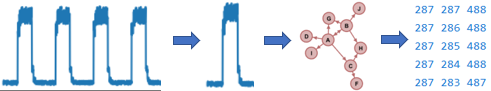
\includegraphics[width=13cm]{fig/tsToNet/tsToCsv}
	\caption{Umwandlung einer Zeitreihe in Netzwerk}
	\label{img:tsToNet}
\end{figure}
\workTodo{Das Netzwerk aus der Grafik noch ab�ndern}
